\documentclass[final,3p,times,twocolumn]{elsarticle}
%% The amssymb package provides various useful mathematical symbols
\usepackage{amssymb}
\usepackage{graphicx} %[trim]
%\usepackage{tikz}
%\usepackage{xcolor}
%\usepackage{multimedia}
\usepackage{media9}

\begin{document}

\begin{frontmatter}

\title{Robotics101}

\author{Sergio Azizi}

\begin{abstract}
Introduction to the problem, MDP's, etc.
\end{abstract}

\end{frontmatter}

%Main text
\section{Microcontroller}
\begin{figure}[h!]
\centering
\caption{Arduino Uno}
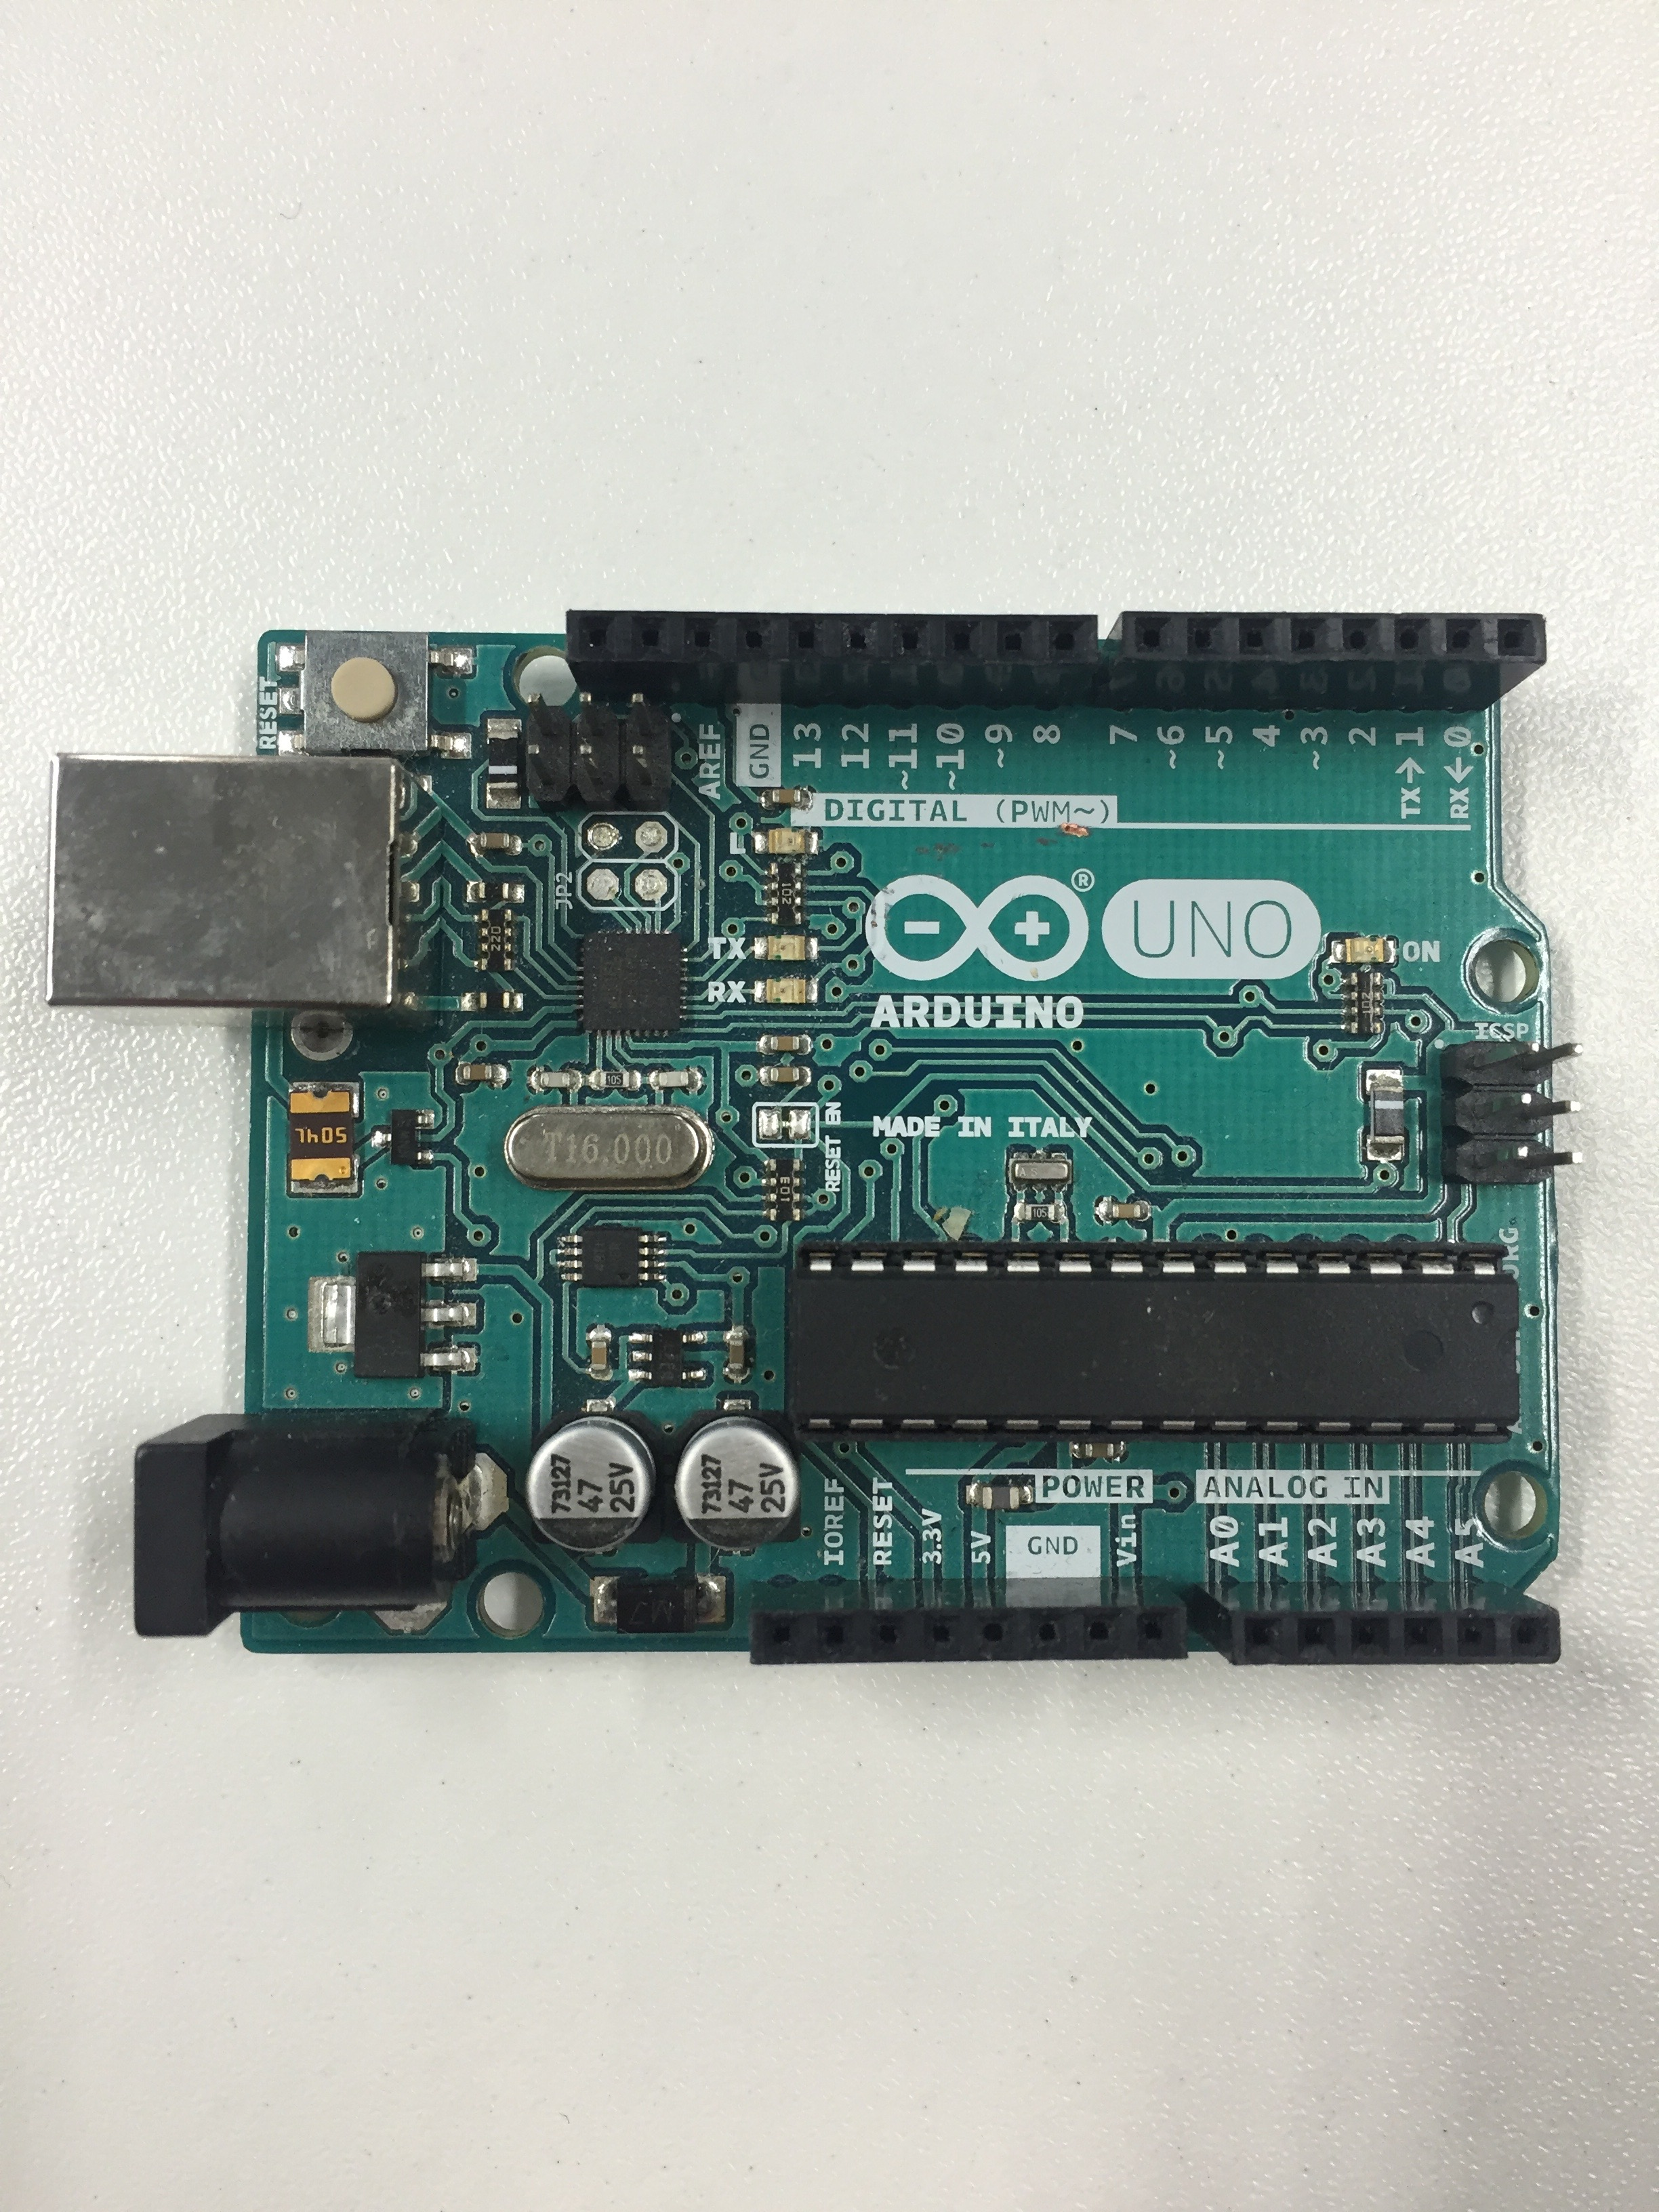
\includegraphics[trim={0 28cm 0 30cm}, clip, width=3in]{./media/microController.jpg}
\label{fig:MicroController}
\end{figure}

\section{Mission}
Build a robot that that will follow a light source while avoiding obstacles
...complete

\includemedia[
  width=0.4\linewidth,
  height=0.3\linewidth,
  activate=pageopen,
  addresource=./media/lightFollow.MP4,
  flashvars={source=./media/lightFollow.MP4}
]{}{VPlayer.swf}

\section{Journey}
The only actuators needed were two brushless DC motors.
Each motor requires a current of 0.5 amps and a voltage of at least 6V.
However, the Arduino Uno is only capable to providing 0.4 amps and 5 volts.
Solution:
With a motor driver circuit and a switch that operates at the Arduino current/voltage level (on means 5V, of means 0V),  I control the necessary amps and volts to change directions of the rotation.
Motor Driver:
Basically, the Driver is is arranged like an H-Bridge. When the switch is turned on (supplying 5V to Arduino), pin 2 will close, causing the motor to rotate clockwise. Similarly, when the switch is turned off (by supplying 0V), pin 3 will close and the motor will rotate in the opposite direction.

\section{Sensors}
A sensor detects changes in its environment (through through its physical properties, eg a thermistor changes its internal resistance with changes in temperature) and passes this information on to the microcontroller through changes in voltage.
We can then program the microcontroller to interpret these voltages however we like (for example, when temperature becomes unusually high, light an LED to signal that something unusual is happening or trigger some other process).
A sonar, for obsticle avoidance (yes, like a bat).
\begin{figure}[h!]
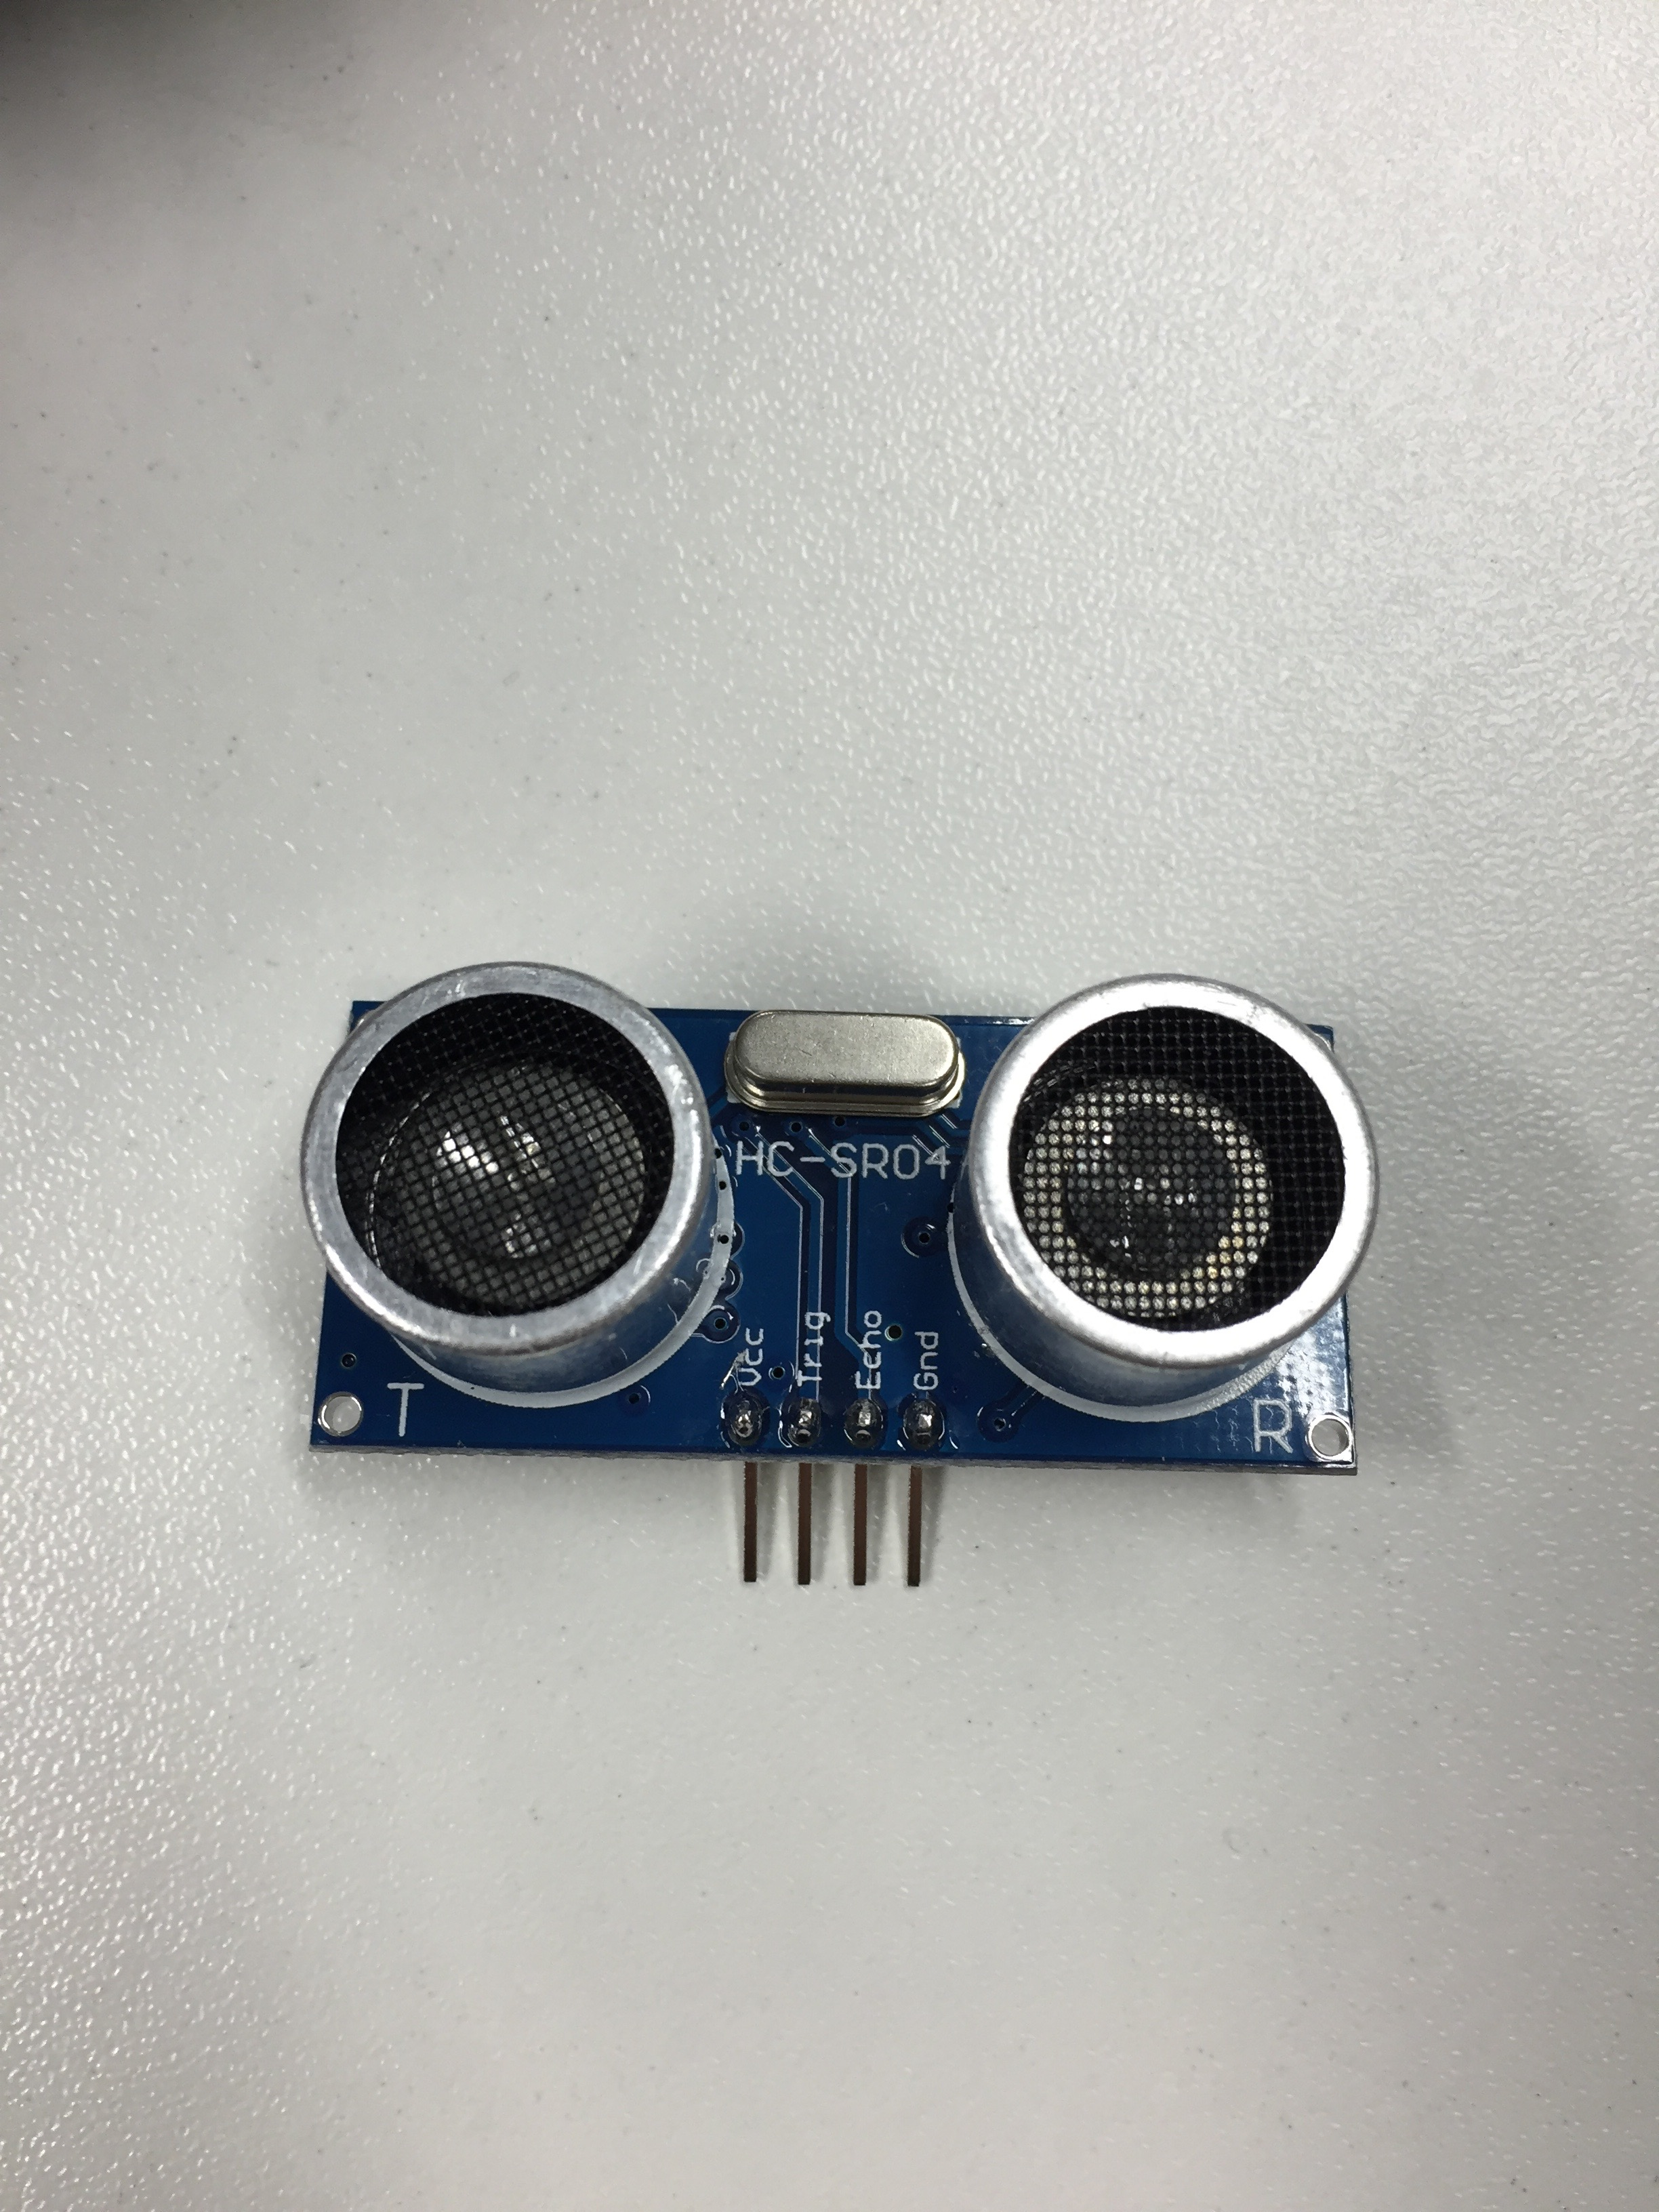
\includegraphics[trim={14cm 30cm 14cm 50cm}, clip, width=3in]{./media/Sonar.jpg}
\end{figure}
A Light Dependent Resistor (LDR) for detecting changes in light.

\section{Assenbly}
2 DC Brushless motors, 2 wheels, 

\end{document}
